%{\normalfont\initfamily \fontsize{12mm}{12mm}\selectfont D}
\begin{multicols}{2}
  \cappar Estimados leitores, neste último número do nosso primeiro
  ano na revista, quis escrever este artigo para vos contar com algum
  pormenor como é que se está a desenvolver a história desta
  revista. Chamo-me María e sou coordenadora da revista. Há pouco mais
  de um ano, a empresa Saema ofereceu-me a possibilidade de colaborar
  na criação de uma revista científica–divulgativa, onde tivéssemos a
  oportunidade de mostrar como a matemática é uma ferramenta preciosa
  em temas de engenharia, especialmente em temas de energia e águas,
  que são as especialistas na empresa Saema. Quando comecei, já estava
  o nosso colega Bartlomiej Skorulski, também doutor em matemática, a
  montar o design da revista e a escrever os primeiros artigos sobre a
  catenária. Estávamos emocionados por participar num projeto em que o
  nosso principal objetivo era dar, aos nossos leitores, qualidade
  informativa.  Como sabem, atualmente, a nossa revista tem várias
  secções. A primeira secção denominamos ''Nada é Impossível” e hoje
  entrei eu nela. Esta secção queria que, vocês e às vezes nós,
  falássemos da nossa experiência com as ciências, de como vemos as
  ciências em Angola, e principalmente fazer ver que não há nada
  impossível que não se possa fazer com força e vontade. A segunda
  secção intitulada ''Solução em ação” estava destinada às pessoas que
  fazem possível que hoje a Saema esteja aqui. Recorremos a várias
  experiências de funcionários da Saema e de amigos da Saema, para nos
  contarem o seu quotidiano, e enviarem mensagens ao povo angolano. A
  secção de Matemática em engenharia é o coração da revista. É
  propriamente o que mais a define, e aí tentamos explicar e aproximar
  a matemática escrita a postes de luz, a canos e a ondas de uma boa
  música como a de Bonga. A secção de Informática em Engenharia, foi
  concebida porque cada vez mais é importante ter alguns conhecimentos
  de informática que deem possibilidades para poder criar aquelas
  coisas que lhe passam pela cabeça. A programação está imersa no
  dia-a-dia, e achamos que é importante fazer com que participe nela
  para entender melhor o mundo. Neste primeiro ano dedicámo-nos a uma
  linguagem funcional e muito potente que é Otave. Espero que tenha
  desfrutado dele etenha podido seguir as diferentes práticas. Neste
  último número do ano, colocamos vários problemas para desenvolver
  com Otave.  Esperamos que os aproveite! Na secção de “Novidades”
  contamos algumas curiosidades que considerámos que eram dignas de
  lhes dedicar um artigo para compartilhar com todos vocês. E a última
  secção, ''Pensar a Brincar”, onde nos permitíamos sair ao pátio para
  brincar imaginativamente.  Como sabem, a Saema promove um grupo de
  xadrez e quisemos fornecer algumas informações de xadrez para apoiar
  o grupo e fazer um apanhado deste apaixonante mundo que é tão
  popular em todo o mundo.  Muitos de vocês são seguidores do nosso
  facebook da revista. Está a ser muito divertido partilhar um artigo
  ou uma foto. Obrigada por nos compartilharem, e espero que continuem
  a fazê-lo nos meios sociais.
 
  \begin{figurebox}
       \centering
  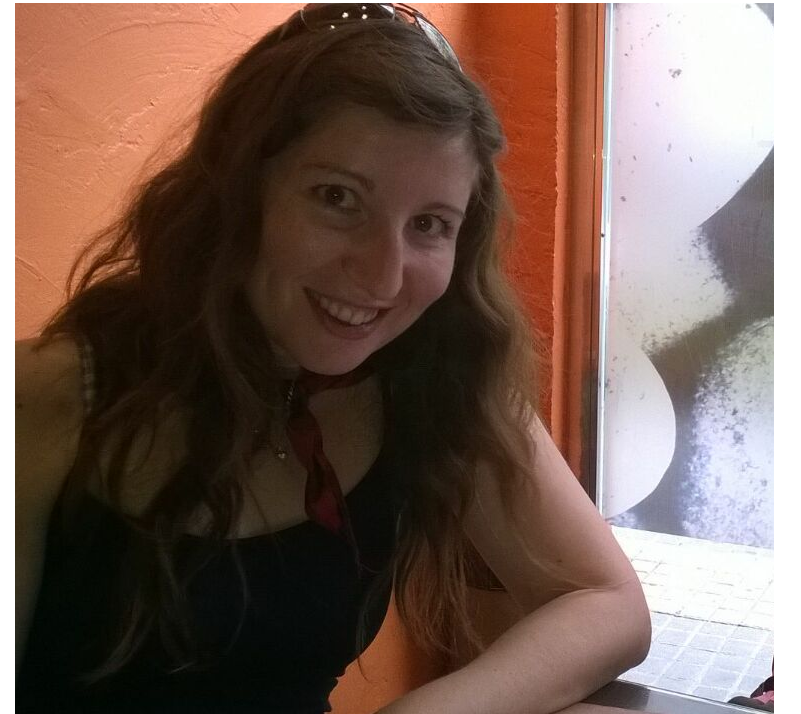
\includegraphics[scale=0.29]{maria.png}\\
    María José Peláez Montalvo\\ 
    {\small Coordenadora Revista Soluçoes}\\
    \vspace{1pt}
    %\vspace{0.1\textheight}
  \end{figurebox}
\vspace{1cm}

A criação desta revista teve várias etapas. A primeira etapa de
discussão, de seleção de temas pela equipa. Uma etapa de estudo, de
procura de informação e de criação. Uma terceira etapa de revisão e
discussão. Uma quarta etapa de maquetação. Uma etapa de revisão final,
e chega o momento culminante: a impressão da revista.

Em aralelo, vamos partilhando os conteúdos em formato digital, onde
vos damos mais informações, como sejam aplicações, uma página web
desenhada por nós para poderem jogar com os conceitos, ou usá-los para
os ensinar a outros, e os códigos dos programas e gráficos expostos na
revista. E a etapa final serve que vos chegue e que a recebam, tal
como me disseram, com um sorriso.  Gostaríamos que nos escrevessem
mais, que nos fizessem saber sobre os temas que vos interessam, que
inquietudes têm e se conhecem novidades importantes de mencionar:
enviem-nos tudo. Estamos recetivos e felizes por poder conhecer-vos, e
tentar dar-vos mediante a nossa revista uma infinita satisfação de
amor à ciência.  Aproveito para vos desejar um feliz 2015 em nome de
toda a minha equipa. Continuem a sonhar e a recordar que um grande
contributo é, afinal, uma soma de pequenas contributos.


\end{multicols}
\vspace{2cm}
      \centering
  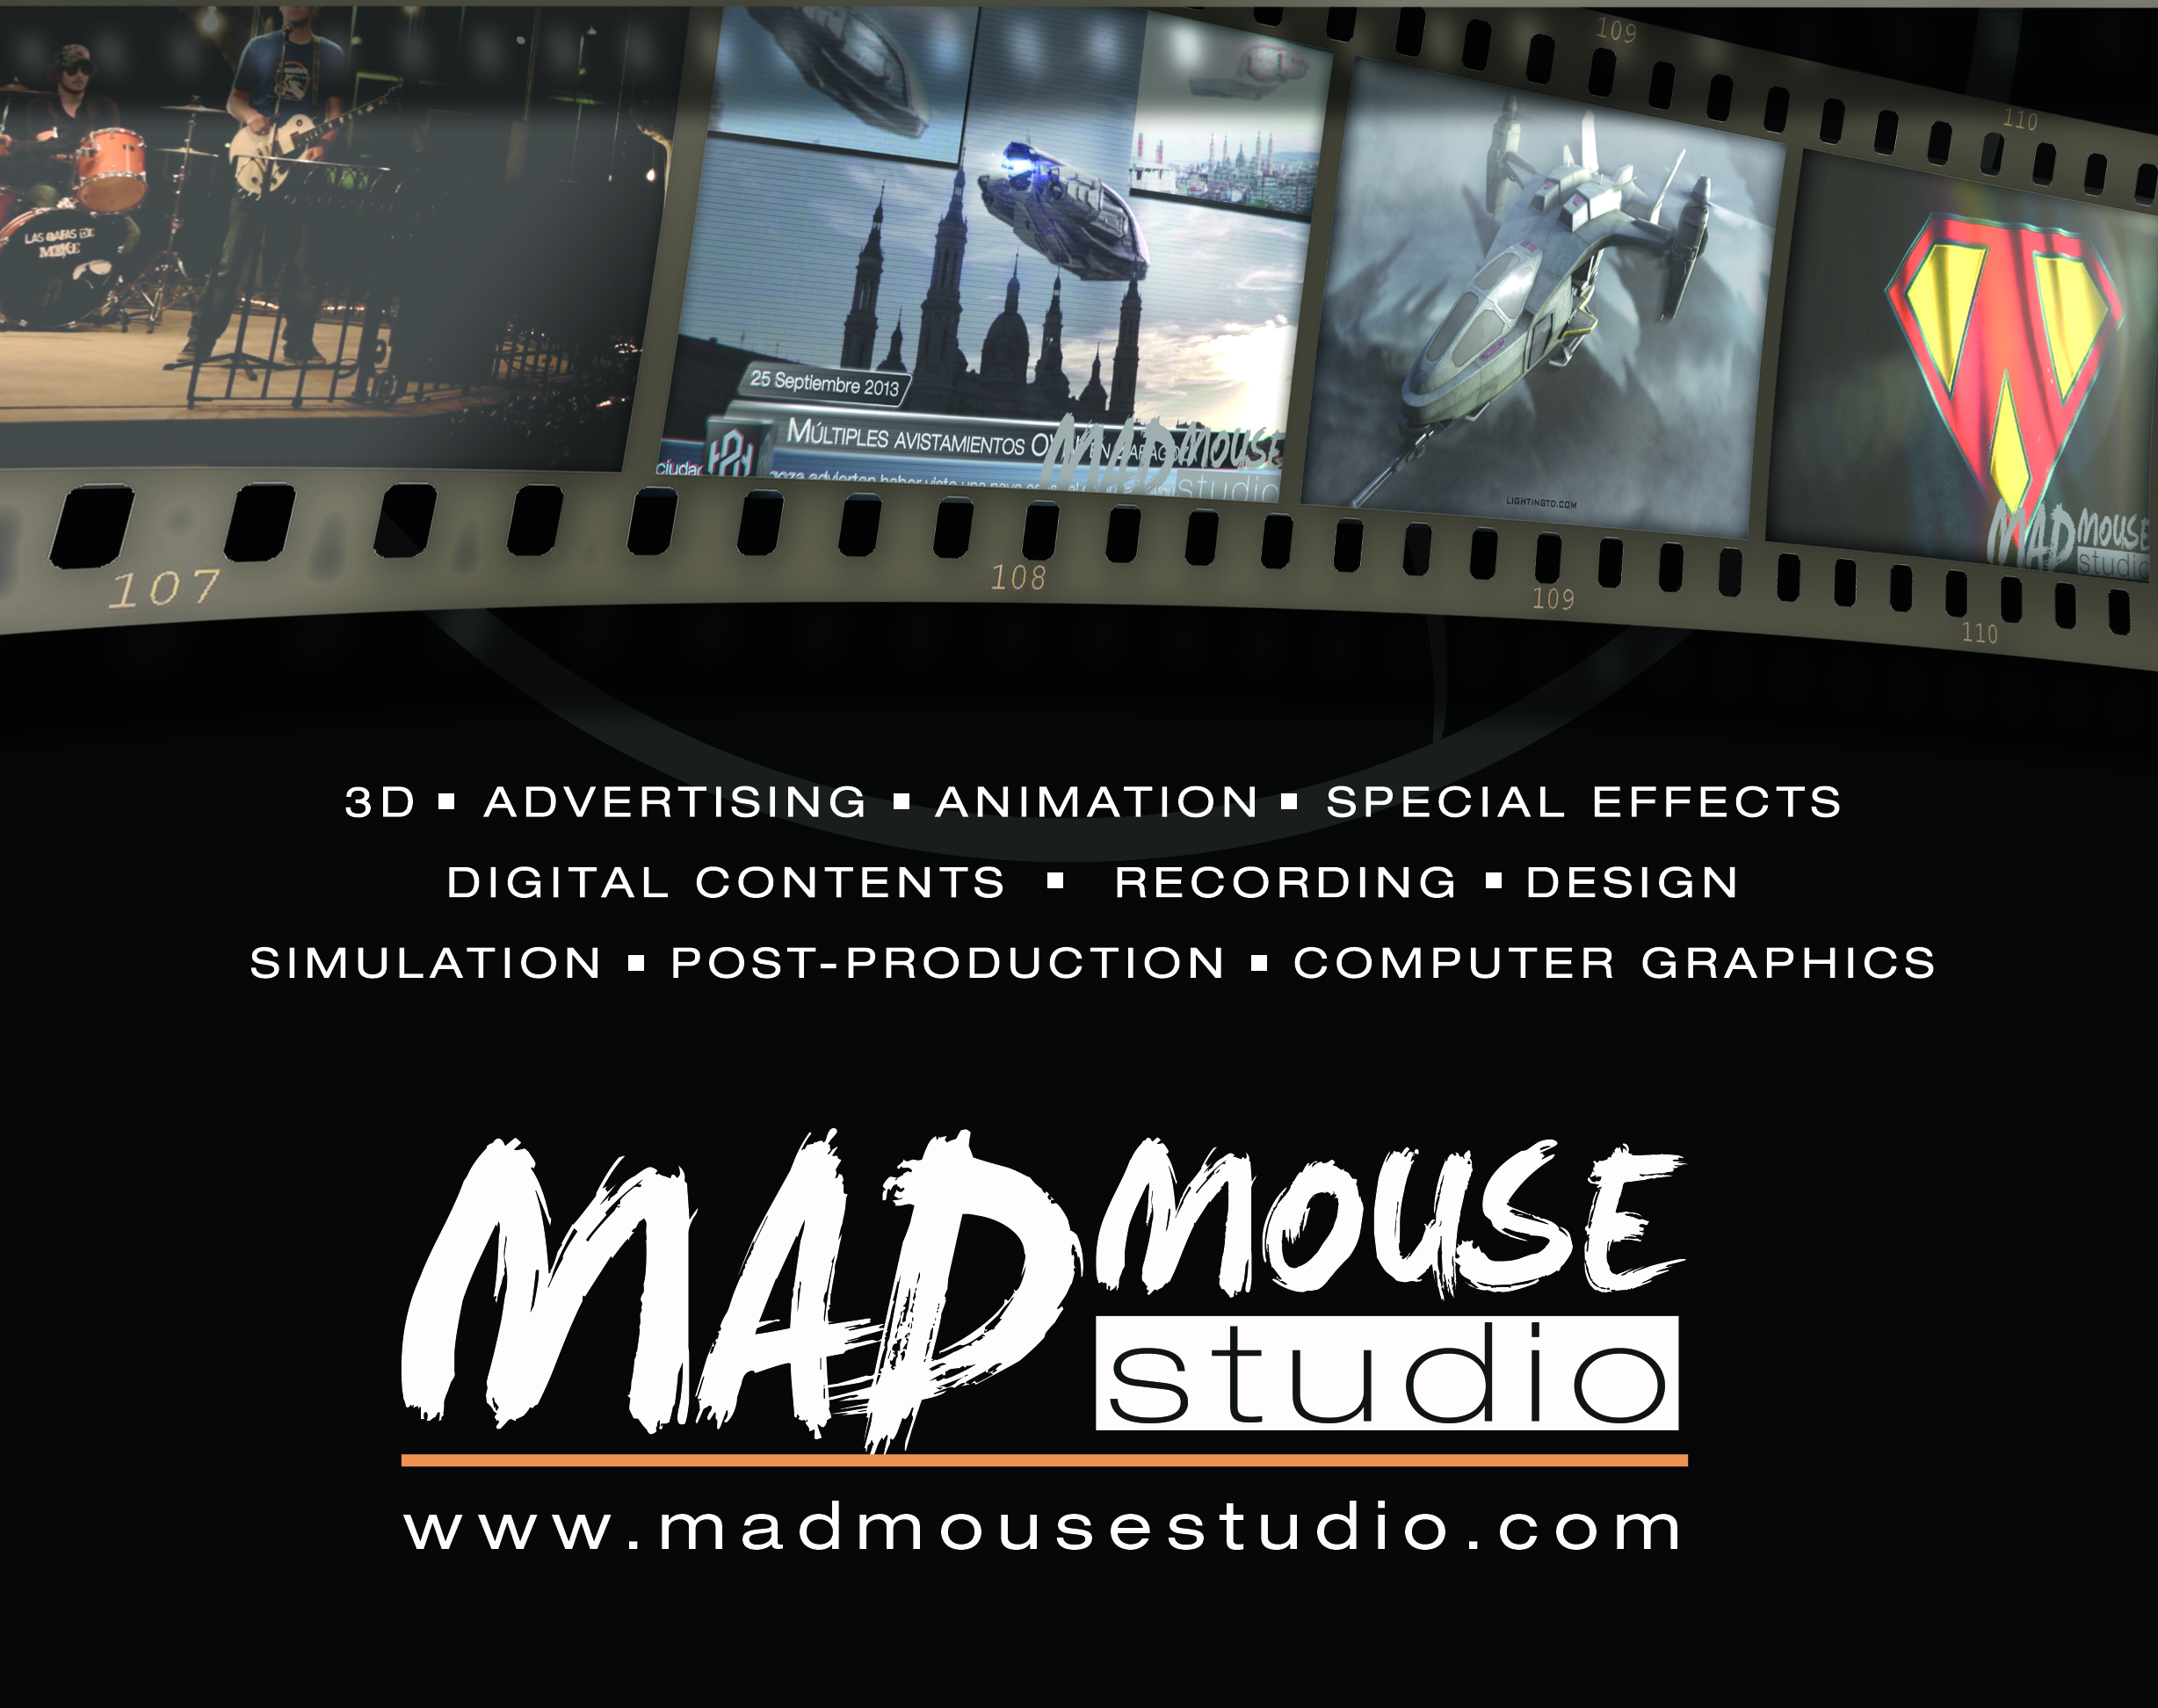
\includegraphics[scale=0.8]{pubmm.png}\\
 \newpage
%%% Local Variables: 
%%% mode: latex
%%% TeX-master: "nadaesimposible"
%%% End: 


